\chapter{Implementation}
\label{chp:implementation} 

\section{Introduction}

This chapter presents four implementations that were developed during this project. The implementations are as follows:

\begin{description}[align=right, labelwidth=5cm]
	\item[Robot software in \ac{ROS}] The robot's operating system. 
	\item[Motor Control Firmware] Translate velocity commands to wheel 
	\item[Android Application] gsdg
	\item[Operator Control Station] sgsd
\end{description}

\section{ROS Integration}

Implementation procedure for mobile robot:

\begin{itemize}

	\item Decide on ROS message interface.
	\item Write interfaces for the motor drivers.
	\item Create a description of the physical structure and properties of the robot in \ac{URDF}. 
	\item Extend the model to enable simulation in Gazebo.
	\item Publish coordinate transform data via \textit{tf} and visualize it in rviz.
	\item Add sensors, with driver and simulation support.
	\item Apply algorithms for navigation and other functionality. 

\end{itemize}

\section{Modeling}

\subsection{Introduction}



\subsection{Physical Dimensions}

\begin{figure}[h]
	\centering
	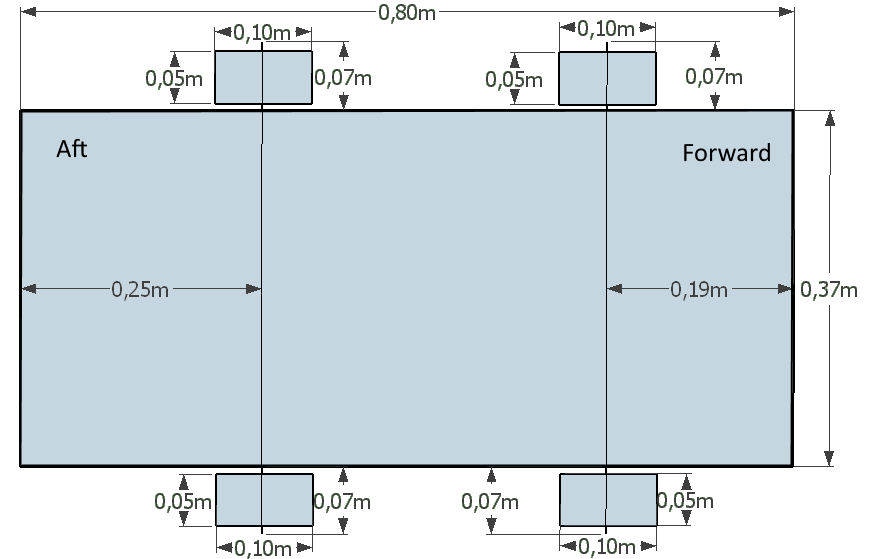
\includegraphics[width=0.85\textwidth]{robotFootprint2}
	\caption{The robot footprint. Dimensions are used for the navigation planners and for modeling. }
	\label{fig:robotFootprint}
\end{figure}

The inertia tensor:

\begin{equation}
    	I = \begin{bmatrix}
    	I_{xx} & I_{xy} & I_{xz} \\[0.3em]
    	I_{yx} & I_{yy} & I_{yz} \\[0.3em]
    	I_{zx} & I_{zy} & I_{zz}
    	\end{bmatrix}
\end{equation}

Inertia tensor for a solid, uniform cylinder where the radius $r$ is measured in parallel to the $x - y$ plane, and $h$ is parallel to the $z$ axis:
\begin{equation}
I_{cylinder} = \frac{1}{12}m \begin{bmatrix}
	(3 r^2 + h^2) & 0 & 0 \\[0.3em]
	0 & (3 r^2 + h^2) & 0 \\[0.3em]
	0 & 0 & r^2
	\end{bmatrix}
\end{equation}

Inertia tensor for a solid, uniform cuboid. The subscript of $l$ indicates which axis $l$ is measured along:
\begin{equation}
I_{cuboid} = \frac{1}{12}m \begin{bmatrix}
	(l_y^2 + l_z^2) & 0 & 0 \\[0.3em]
	0 & (l_x^2 + l_z^2) & 0 \\[0.3em]
	0 & 0 & (l_x^2 + l_y^2)
\end{bmatrix}
\end{equation}

\subsection{Coordinate Frames}

\begin{figure}[h]
	\centering
	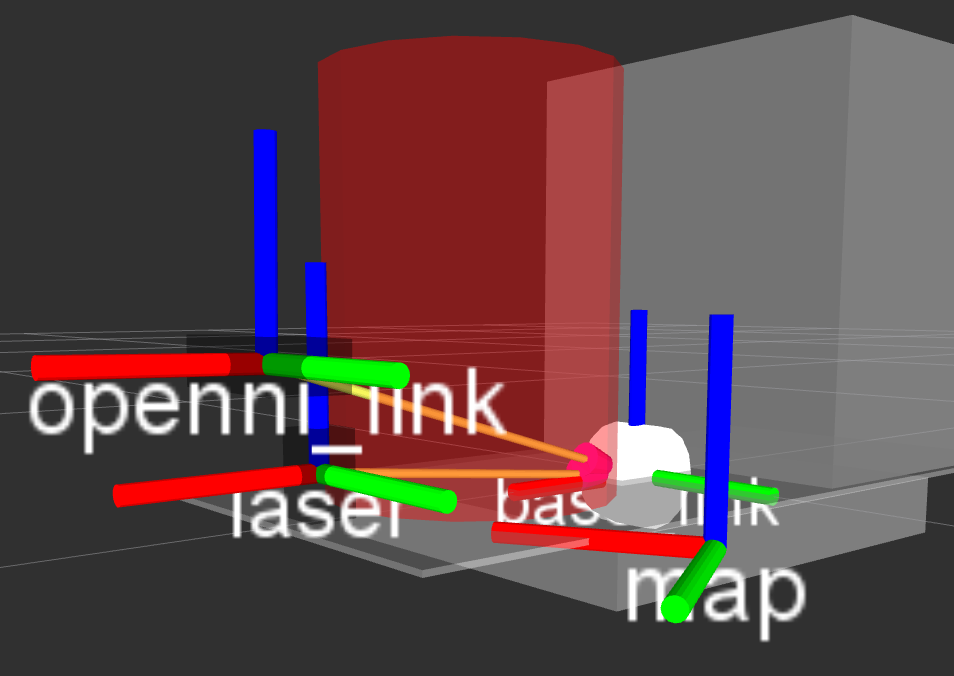
\includegraphics[width=0.5\textwidth]{sensor_frames}
	\caption{Robot model with frames for laser, Kinect, robot base and map. }
	\label{fig:sensor_frames}
\end{figure}

\begin{figure}[h]
	\centering
	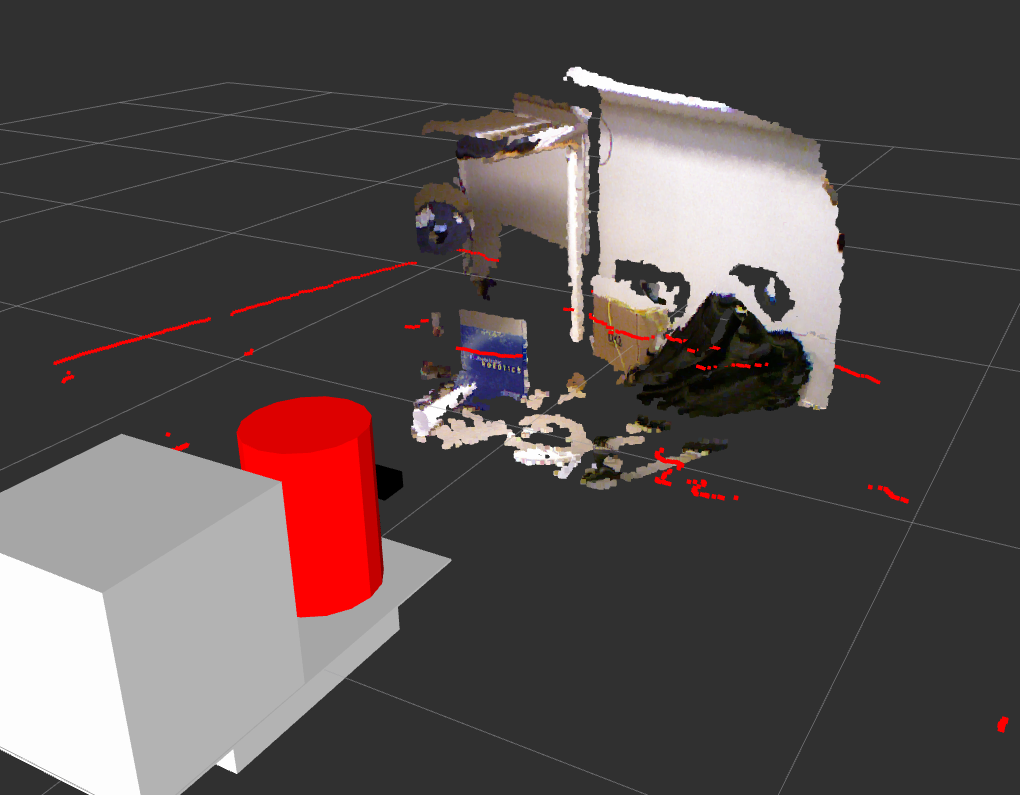
\includegraphics[width=0.5\textwidth]{sensors_in_frame}
	\caption{Sensor input placed with correct transformations from \textit{base\_link}. }
	\label{fig:sensors_in_frame}
\end{figure}


\section{Simulations}

Robot simulation was done in Gazebo, a simulation tool with good interfaces to \ac{ROS}. The same \ac{ROS} graph was used for both the simulated and real version of the robot, except from the sensors and actuators, and some minor parameter changes. 

\section{Motion Control}

\section{ROS Nodes for Motion Control}


\subsection{Velocity Command Sources}

There are four ways to control the robot:

\begin{itemize}
	\item Local keyboard input.
	\item Wireless teleoperation from the \ac{OCS}.
	\item Wireless teleoperation from a hand-held Bluetooth device.
	\item Commands from the navigation stack in \ac{ROS}.
\end{itemize}

\begin{figure}[h]
	\centering
	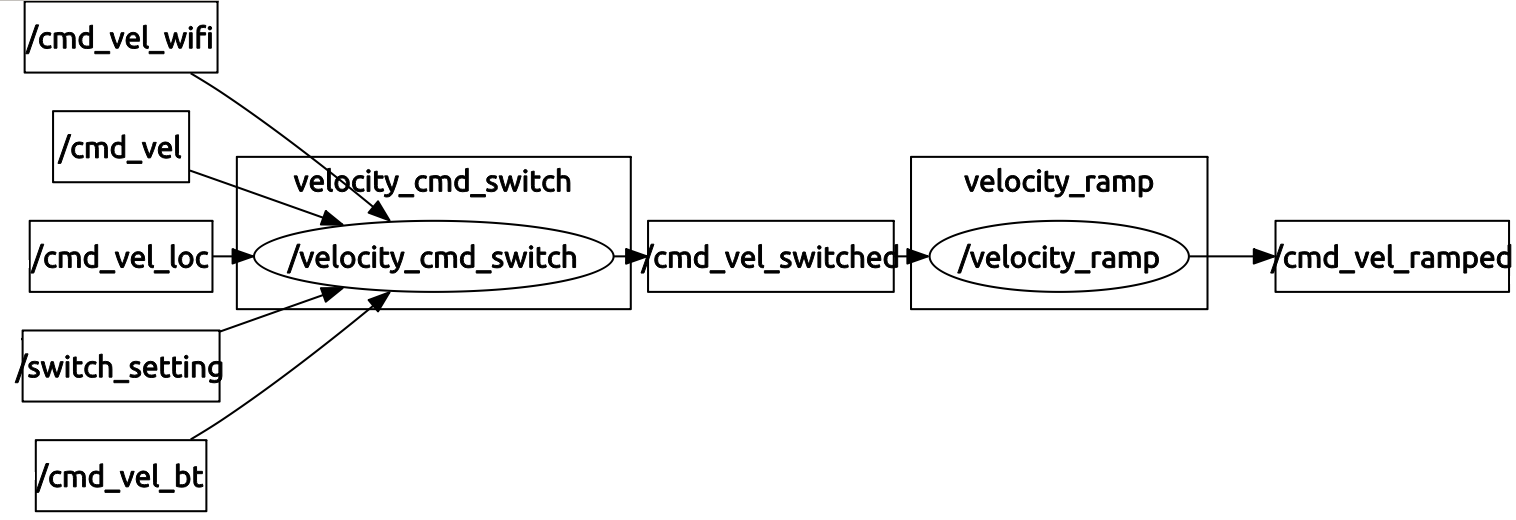
\includegraphics[width=1\textwidth]{velocity_command}
	\caption{Nodes and topics for motion control. }
	\label{fig:move_base_nodes}
\end{figure}

\begin{figure}[h]
	\centering
	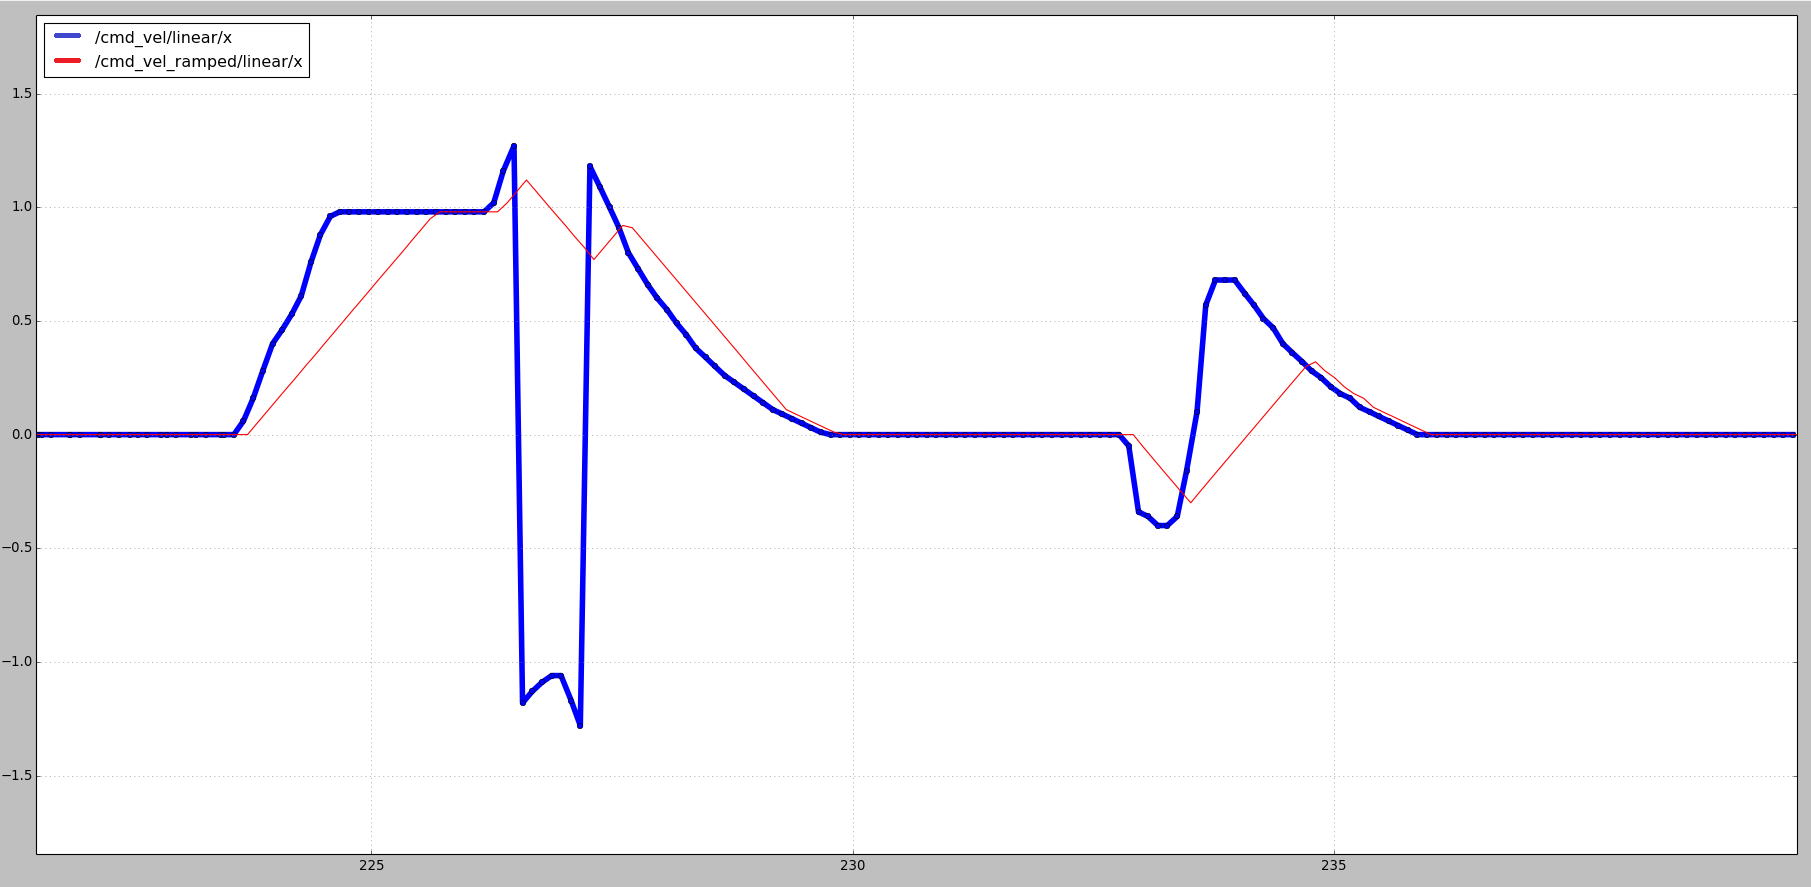
\includegraphics[width=1\textwidth]{velocity_ramp_cropped}
	\caption{Velocity command ramping. The blue line represents commands entering \textit{velocity\_ramp}, while the red line shows the acceleration constrained output command.}
	\label{fig:velocity_ramp}
\end{figure}

\subsection{Motor Control Card Firmware on XMEGA A3BU}

XMEGA A3BU is an evaluation board developed by Atmel. The board has been used in earlier projects on this robot, and the implementation presented here, is based on Petter Aspunviks implementation \cite{aspunvik}. The following paragraphs presents the most significant firmware changes that were made.

The firmware will now receive velocity commands based on the \texttt{geometry\_msgs/Twist} message format in \ac{ROS}, and translate these into the command format used by each motor. Speed settings for each motor is based on \ac{PWM}. 

There were two requirements for this implementation: 
\begin{enumerate}
\item When velocity commands from the operating system are either absent or incomplete, the robot shall stop.
\item The program shall translate linear and angular velocity commands into wheel commands.
\end{enumerate}

\begin{figure}[h]
	\centering
	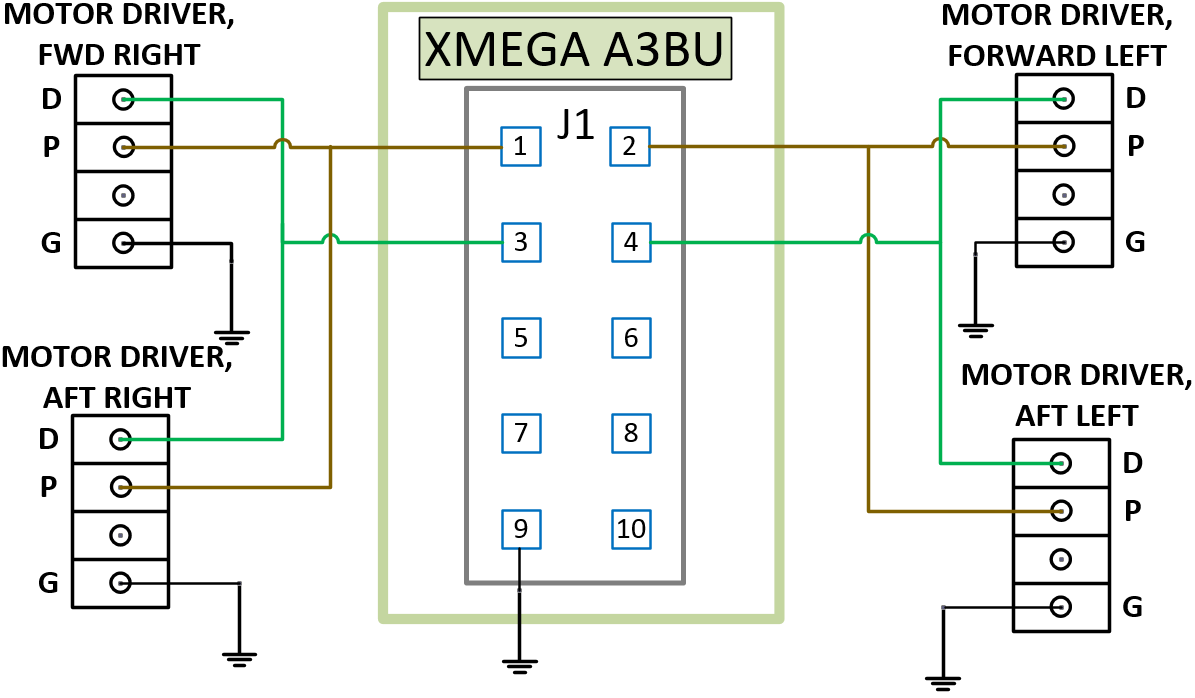
\includegraphics[width=0.9\textwidth]{conn_diag_motors}
	\caption{Connections between each wheel motor driver and the motor control card, XMEGA A3BU. The connections are unchanged from \cite{aspunvik}, except for some improved connection for better short circuit prevention.}
	\label{fig:conn_diag_motors}
\end{figure}

The connections in figure \ref{fig:conn_diag_motors} are the same as in \cite{aspunvik}, except for the installation of more secure connections under the robot. The old connections were insecure, and the risk of short circuits was substantial.

\subsubsection{ROS-Motor Driver Communication}

\begin{figure}[h]
	\centering
	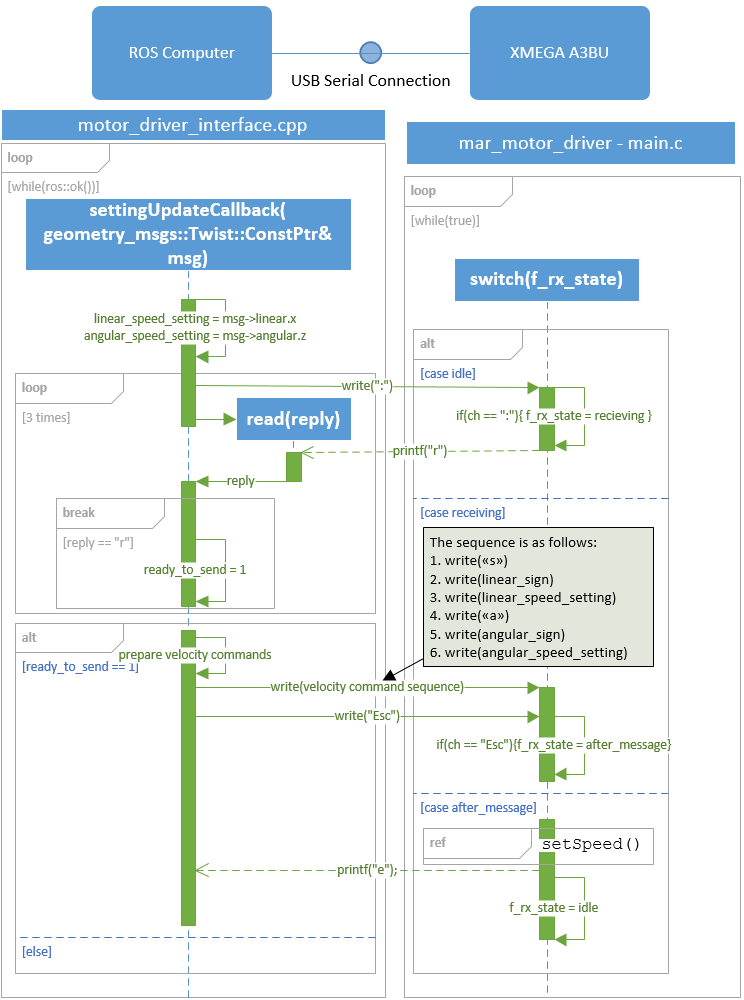
\includegraphics[width=1\textwidth]{motor_cmd_sequence}
	\caption{Velocity command transmission sequence from the \texttt{motor\_driver\_interface} in the ROS computer to the motor control card (XMEGA A3BU).}
	\label{fig:motor_cmd_sequence}
\end{figure}


\subsubsection{From Velocity Commands to Wheel Commands}

Within \ac{ROS}, velocity commands are passed around between nodes in the form of the message \texttt{geometry\_msgs/Twist}. This message type can be viewed as a \textit{struct} with the following contents:

\begin{verbatim}
	Vector3  linear
	Vector3  angular
\end{verbatim}

where each vector contains float values for the directions $x$, $y$ and $z$ with respect to the robot's base frame. Because of the motion constraints of this robot, only \texttt{linear.x} and \texttt{angular.z} are of relevance, and the data which is passed to the motor control card (XMEGA A3BU) is therefore limited to these two values. The motor control card must now translate the linear and angular velocities into wheel speeds. Next, these speeds must be related to a duty cycle for the \ac{PWM} signal which controls each of the four motors.

To perform the translation, it is assumed that the mobile base can be described as a vehicle with differential drive steering. Wheel commands will only distinguish between left or right - not front or aft. Equations of motion which relates angular and linear velocity to wheel velocities can be found in\cite{cook2011mobile}. 

\begin{subequations}\label{eq:subeqns}
  	\begin{align}
	  	\omega &= \dot{\psi} \\
	   	v_{left} &= \omega (R - W/2)\\
	   	v_{right} &= \omega (R + W/2) \label{eq:subeq2}
   	\end{align}
\end{subequations}

In \cite{cook2011mobile}, the parameter $R$ represents the instantaneous radius of curvature of the robot trajectory. This mouthful will be substituted by the linear velocity $v$ in the following equations, because $v = R\omega$ (similar to the linear speed of a wheel). This yields two equations for the wheel speeds, $v_{left}$ and $v_{right}$, based on angular and linear velocity, $w$ and $v$.

 \begin{subequations}%\label{eq:subeqns}
 	\begin{align}
 	v &= R\omega \\
 	v_{left} &=  \frac{2v - \omega W}{2}\\
 	v_{right} &= \frac{2v - \omega W}{2} %\label{eq:subeq2}
 	\end{align}
 \end{subequations}



 \begin{figure}
 	\centering
 	\begin{subfigure}[b]{0.58\textwidth}
 		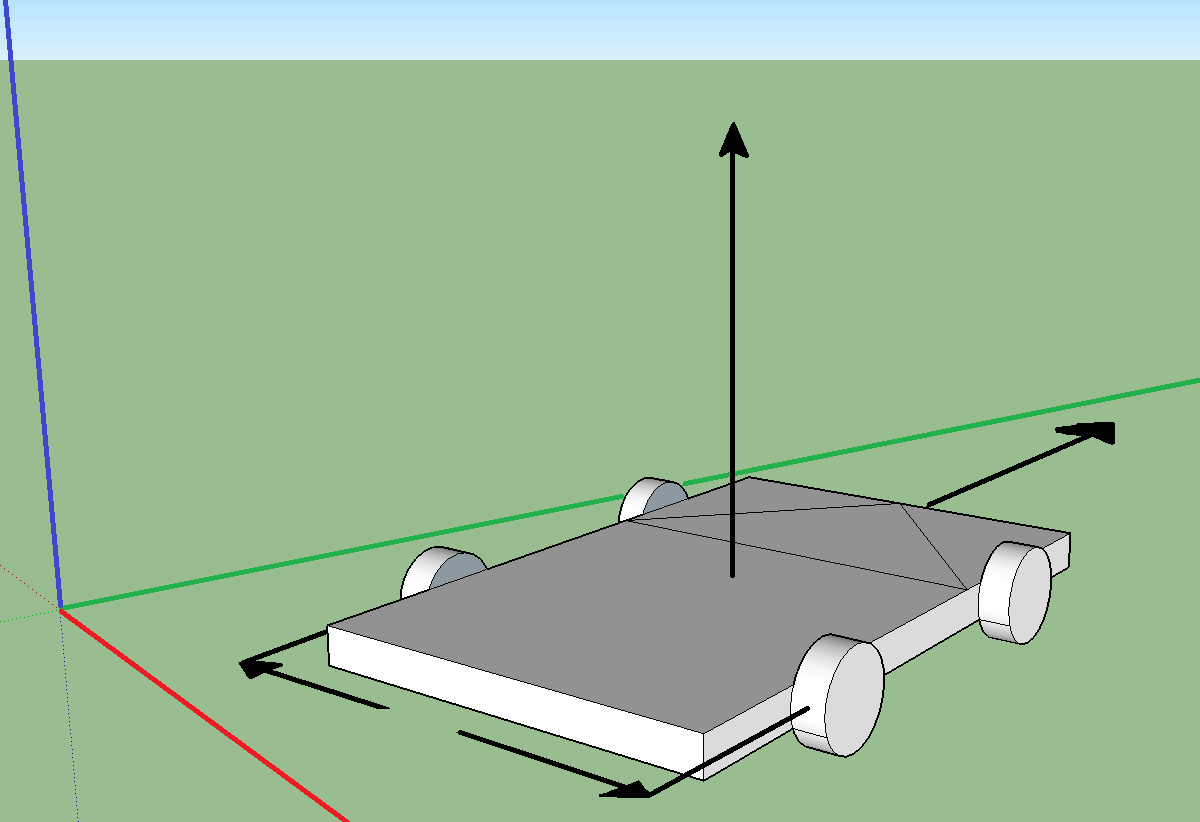
\includegraphics[width=\textwidth]{robot_kinematics}
 		\caption{Differential drive parameters.}
 		\label{fig:robot_kinematics}
 	\end{subfigure}
 	\begin{subfigure}[b]{0.38\textwidth}
 		
 		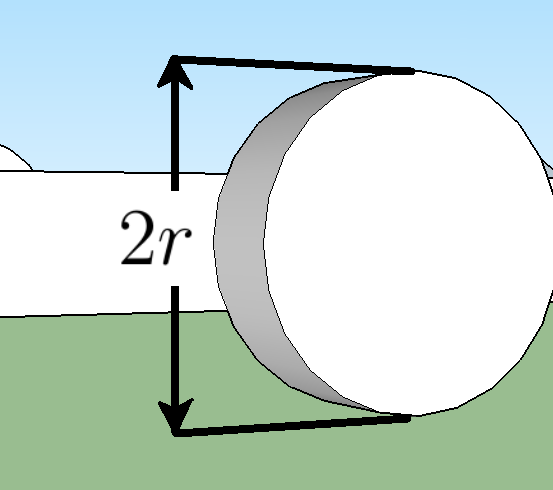
\includegraphics[width=\textwidth]{wheel_diameter}
 		\caption{Wheel diameter.}
 		\label{fig:wheel_diameter}
 	\end{subfigure}
 	\caption{\label{fig:robot_kinematics}Parameters for differential drive kinematics. Note that the frame vectors $\vec{z}$ and $\vec{x}$ refer to the base frame of the robot in this case, and not the world frame.}
 \end{figure}

\section{Operator Control Station (OCS)}

The \ac{OCS} allows an operator to control and monitor the robot through a graphical user interface. \texttt{MainWindow}

\subsection{Graphical User Interface}

A Qt-based \ac{GUI}...

\section{The Hand Held Remote Control - \textit{Robot Leash}}

Because the \ac{OCS} is only partially implemented, an operator will not have access to all the features on the robot. In addition, as a safety precaution a person should be close to the robot at all times, and be ready to pull the plug. Furthermore, it is hard to control a moving robot through the on-board keyboard. These problems were countered by the Android-based remote control, \textit{Robot Leash}. 


\begin{figure}
	\centering
	\begin{subfigure}[b]{0.30\textwidth}
		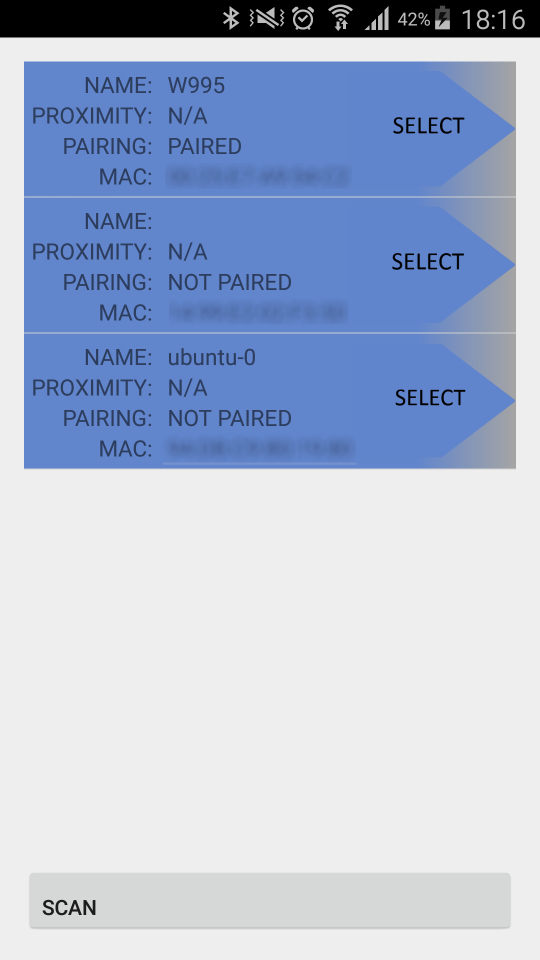
\includegraphics[width=\textwidth]{device_select}
		\caption{First activity with device list.}
		\label{fig:device_select}
	\end{subfigure}
		\begin{subfigure}[b]{0.30\textwidth}
			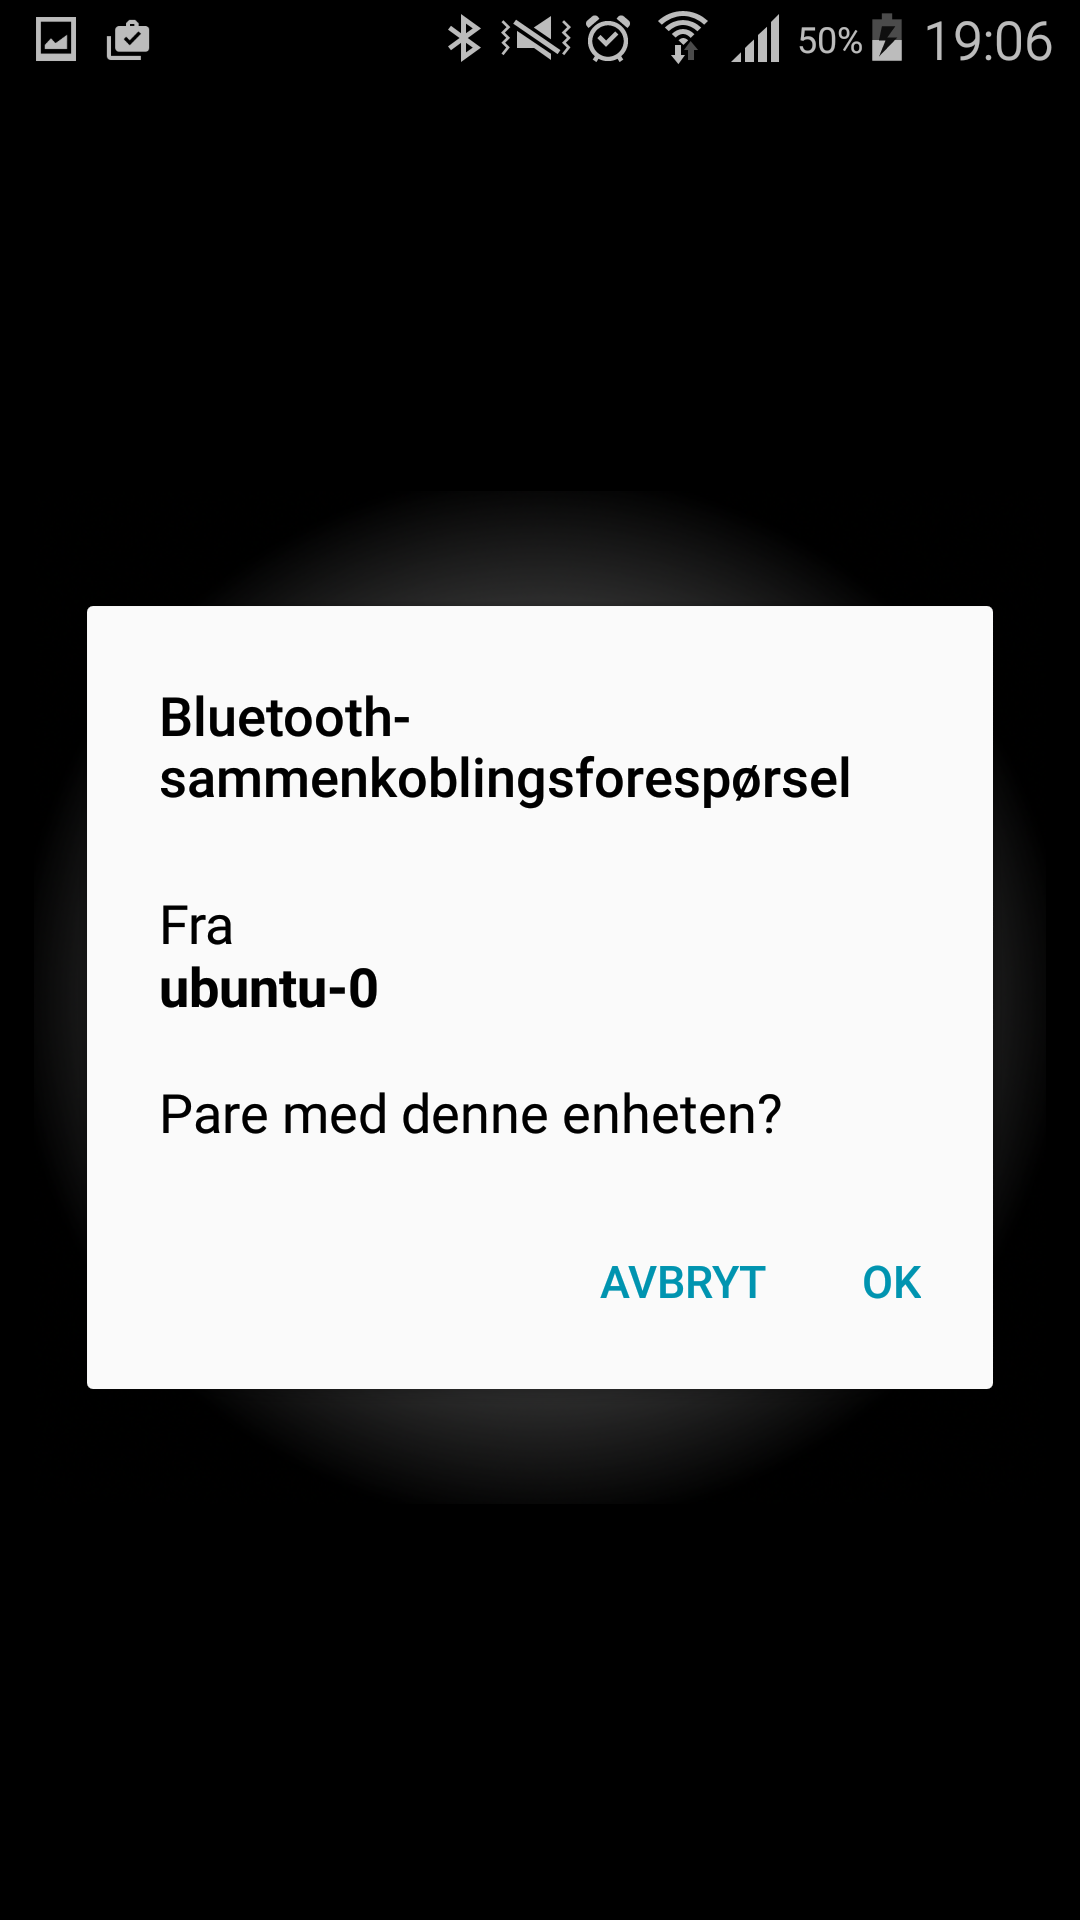
\includegraphics[width=\textwidth]{bt_request}
			\caption{The user is prompted to pair with the robot.}
			\label{fig:bt_request}
		\end{subfigure}
	\begin{subfigure}[b]{0.30\textwidth}
		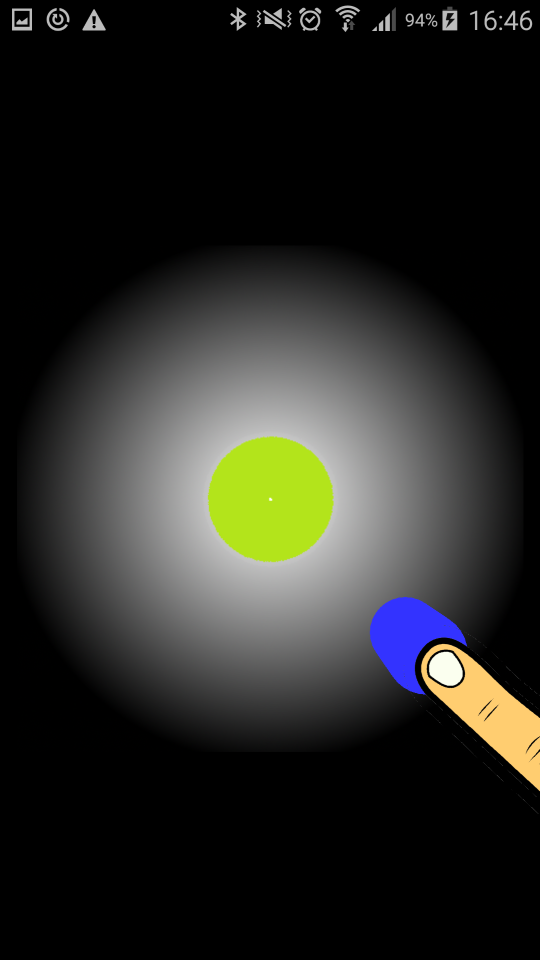
\includegraphics[width=\textwidth]{using_app}
		\caption{Controlling the robot with the stick.}
		\label{fig:using_app}
	\end{subfigure}
	\caption{\label{fig:app_screens}A typical use case for ''Robot Leash''.}
\end{figure}

\subsection{Connecting to the Robot}

\begin{enumerate}
	\item The first screen after scanning for devices. There is no device filtering, and the user can select any device, but only connect through a specific service.
	\item After selecting a device which provides the correct service, the user will be prompted to pair the devices.
	\item The smartphone and the robot is now paired, and velocity commands from the blue control stick are passed to the robot via Bluetooth.
\end{enumerate}

http://developer.samsung.com/technical-doc/view.do?v=T000000117

\begin{sidewaysfigure}[ht]
	\centering
	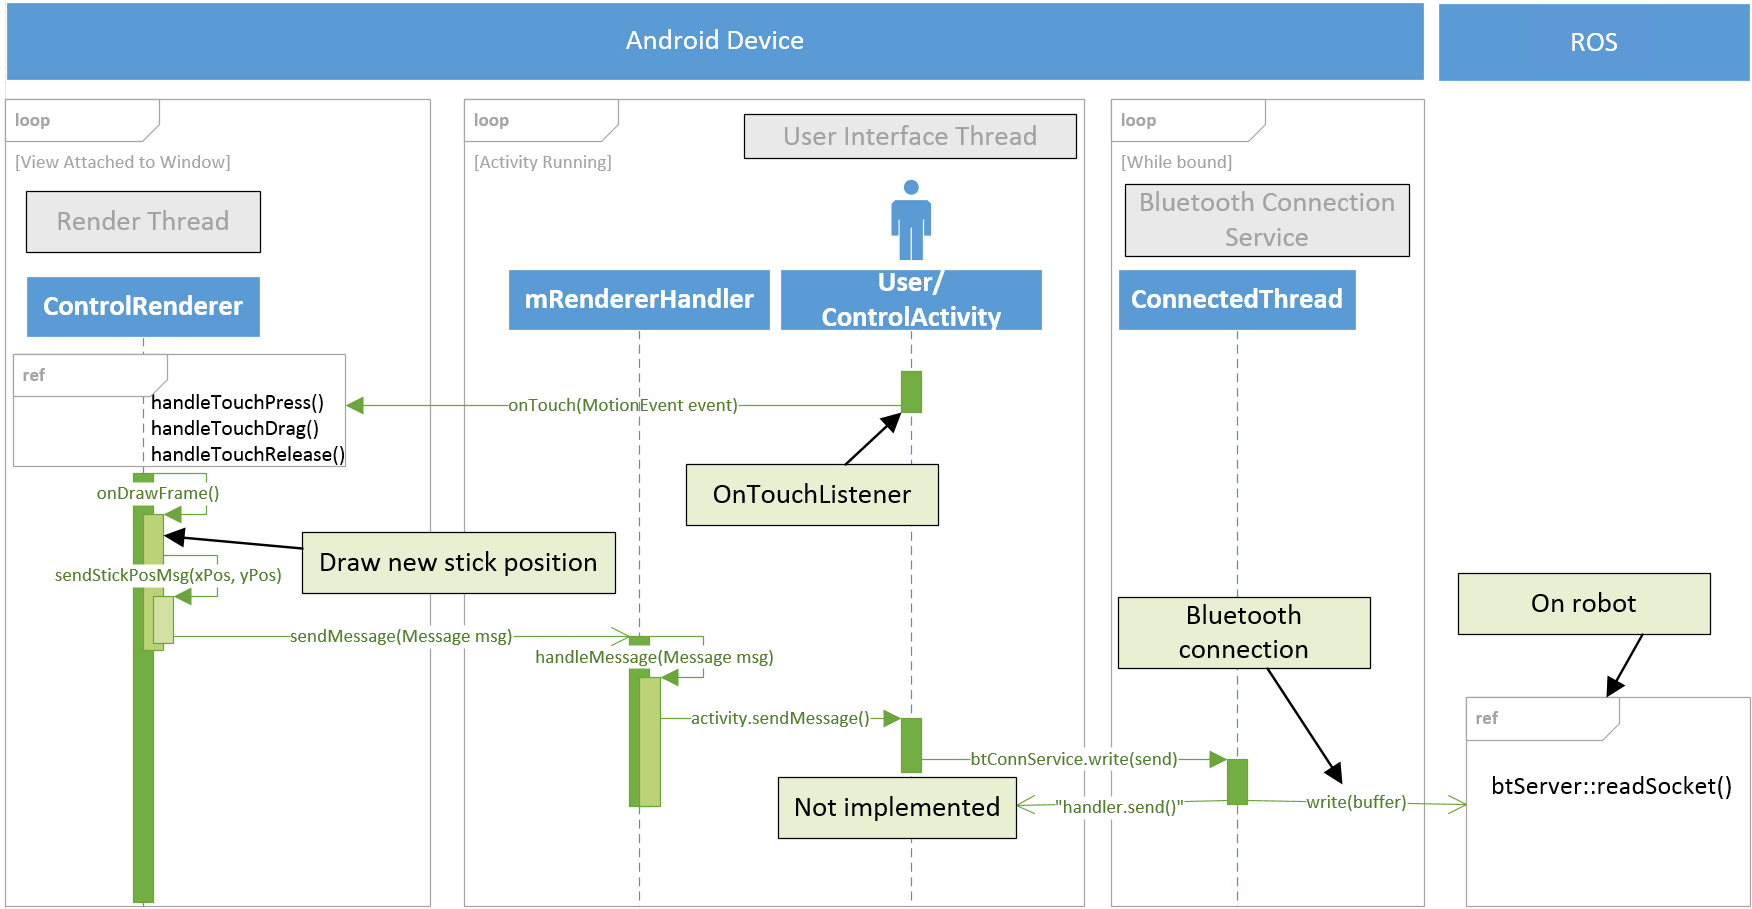
\includegraphics[width=1\textwidth]{android_sequence}
	\caption[This is the caption \newline This is the second line]{\begin{minipage}[t]{.8\linewidth}Sequence diagram illustrating how user touch gestures are detected and propagated \\through the application, before being transmitted as commands to the robot. \end{minipage}}
	\label{fig:android_sequence}
\end{sidewaysfigure}


\section{Mapping}

\section{Navigation}

\subsection{Global Path Planning}

\subsection{Local Path Planning}

\subsubsection{Obstruction Detection}

\begin{figure}
	\centering
	\begin{subfigure}[b]{0.53\textwidth}
		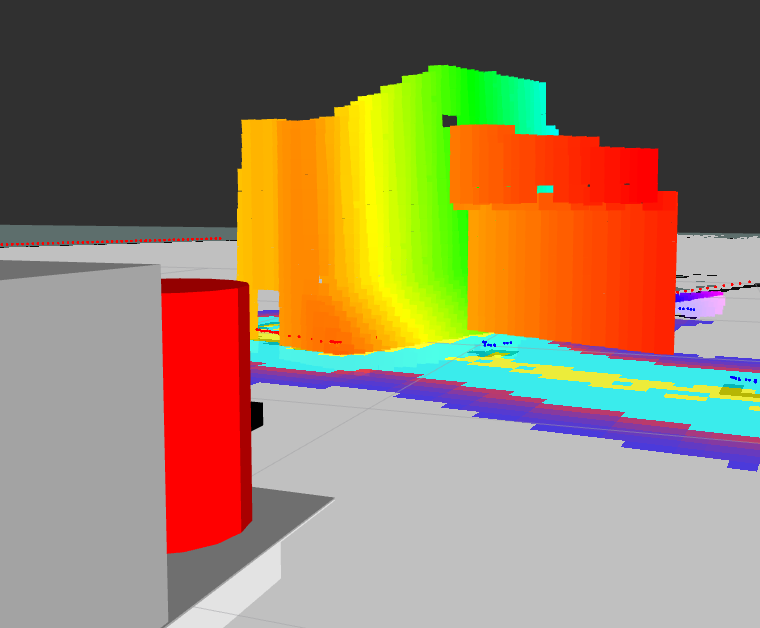
\includegraphics[width=\textwidth]{3d_obstruction1_left}
		\caption{A point cloud representation of the obstruction. Notice how the local costmap is based on the detected point cloud.}
		\label{fig:device_select}
	\end{subfigure}
		\begin{subfigure}[b]{0.45\textwidth}
			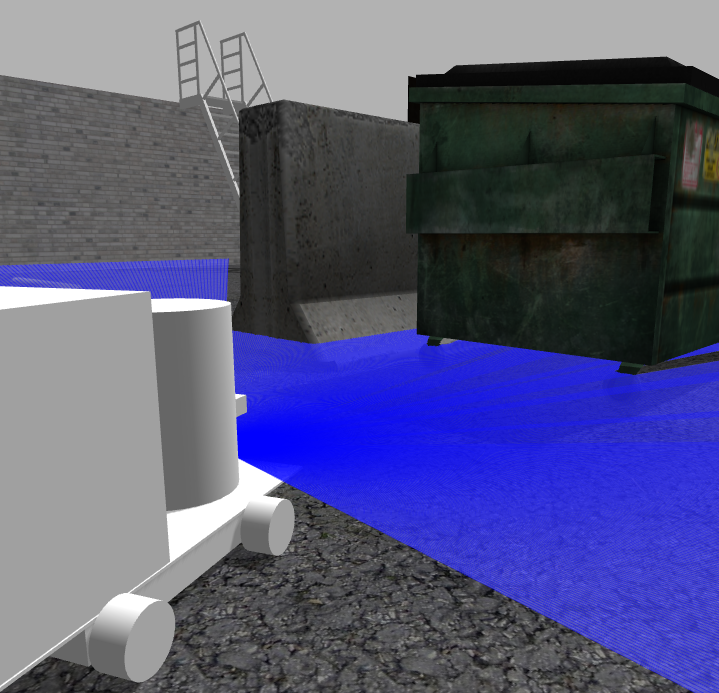
\includegraphics[width=\textwidth]{3d_obstruction1_right}
			\caption{The obstruction in the Gazebo simulator. Notice how the LIDAR only detects the wheels below the container.}
			\label{fig:bt_request}
		\end{subfigure}
	\caption{\label{fig:3d_obstruction1}Detecting obstructions in 3d.}
\end{figure}